\documentclass{beamer}
\usepackage{verbatim}
\usepackage{physics}
\usepackage{amsmath}

\mode<presentation>
{
\usetheme{default}
\usecolortheme{default}
\usefonttheme{default}
\setbeamertemplate{navigation symbols}{}
\setbeamertemplate{caption}[numbered]
}
\usepackage{caption}
\usepackage[english]{babel}
\usepackage[utf8x]{inputenc}
\usepackage{graphicx}

\title[Your Short Title]{Magneto-static Analysis of a Brushless DC Motor}
\author{\small Tom Ginsberg, Brendan Posehn}
\date{}

\begin{document}

    \begin{frame}
        \vspace{0.5cm}
        \titlepage
        \vspace{-1.5cm}
        \begin{center}
            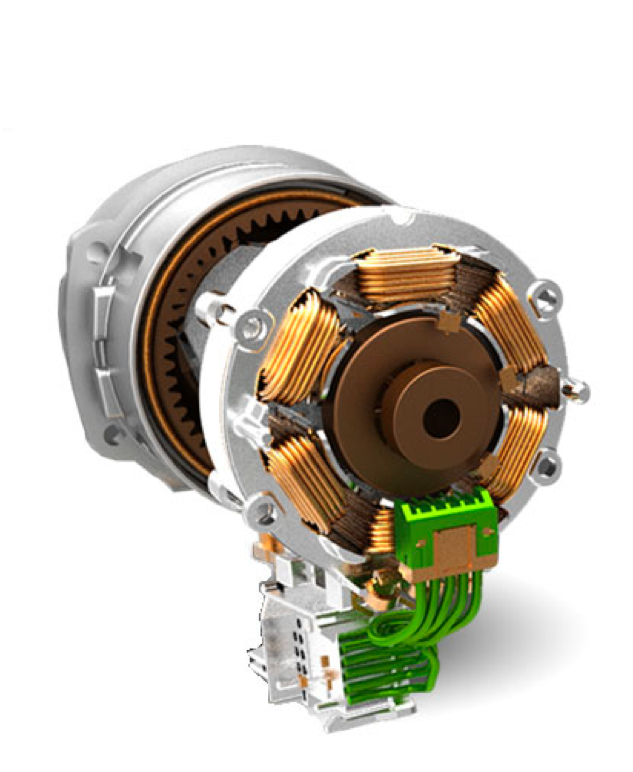
\includegraphics[width=2in]{render.png}
        \end{center}
    \end{frame}

    \begin{frame}{Overview}
        \begin{itemize}
            \item {\large Background}\\
            Brushless DC Motors
            \item {\large Theory}\\
            Magneto-statics, Permanent Magnets, Non Linear Materials, Non Linear FEM
            \item {\large Implementation}\\
            Meshing, Matrix Assembly, Solving, Newton Raphson
            \item {\large Results}\\
            Diagrams, Torques
        \end{itemize}

    \end{frame}
    \begin{frame}{Theory: Magnetostatics in a 2D Cross Section}
        If current is only perpendicular to the 2D plane, then
        \begin{align*}
            &\nabla\times \nu B=J\text{ and }\nabla \times A = B\\
            &\nabla\times \nu \nabla\times A=J \iff \nabla\cdot \nu \nabla A=J
        \end{align*}
        \begin{center}
            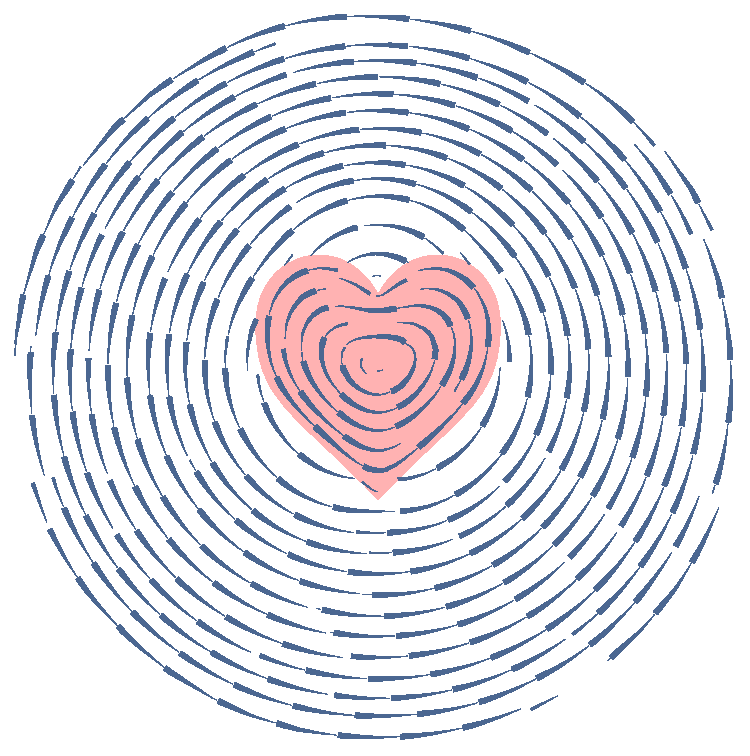
\includegraphics[width=3in]{heartwire.pdf}
        \end{center}
    \end{frame}
    \begin{frame}{Theory: Permanent Magnets}
        Maxwell's Equation's for Permanent Magnets
        \begin{align*}
            B &= \mu H +\mu_0 M_r\text{ and } \nabla \times H = J \implies \nabla \times \nu B=J+\nabla\times \nu\mu_0 M_r\\
            J_m&\triangleq \nabla\times \nu\mu_0 M_r \implies \nabla \times \nu B=J+J_m
        \end{align*}
        \begin{center}
            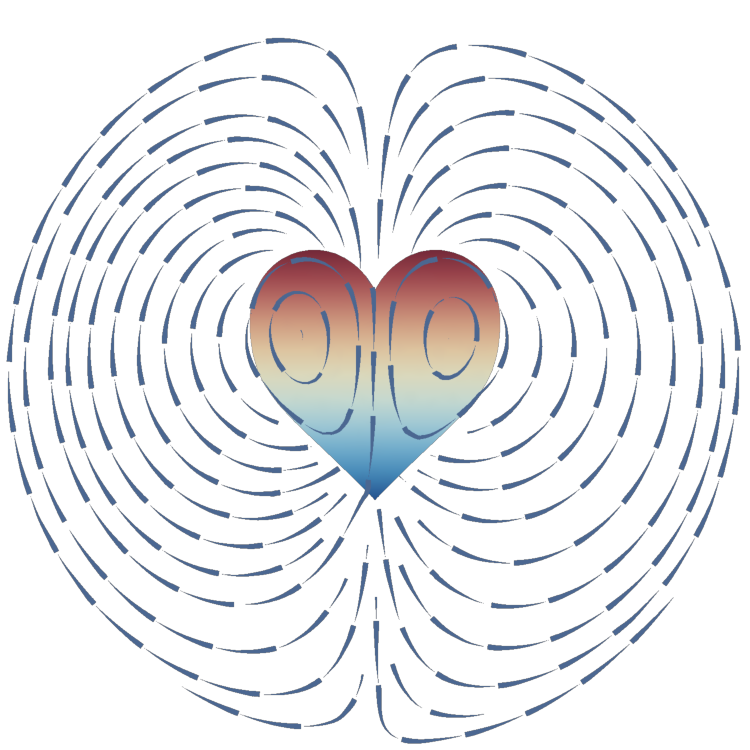
\includegraphics[width=3in]{heartmag.pdf}
        \end{center}
    \end{frame}
    \begin{frame}{Permenant Magnets}
        We use a \textit{2D-coil} model for permanent magnets.
        \begin{itemize}
            \item \textbf{Assumption}: A bar magnet has a similar field to a current carrying coil
            \item \textbf{Heuristic}: Any magnet geometry can be approximated from gluing together curved bar magnets
        \end{itemize}
        \begin{center}
            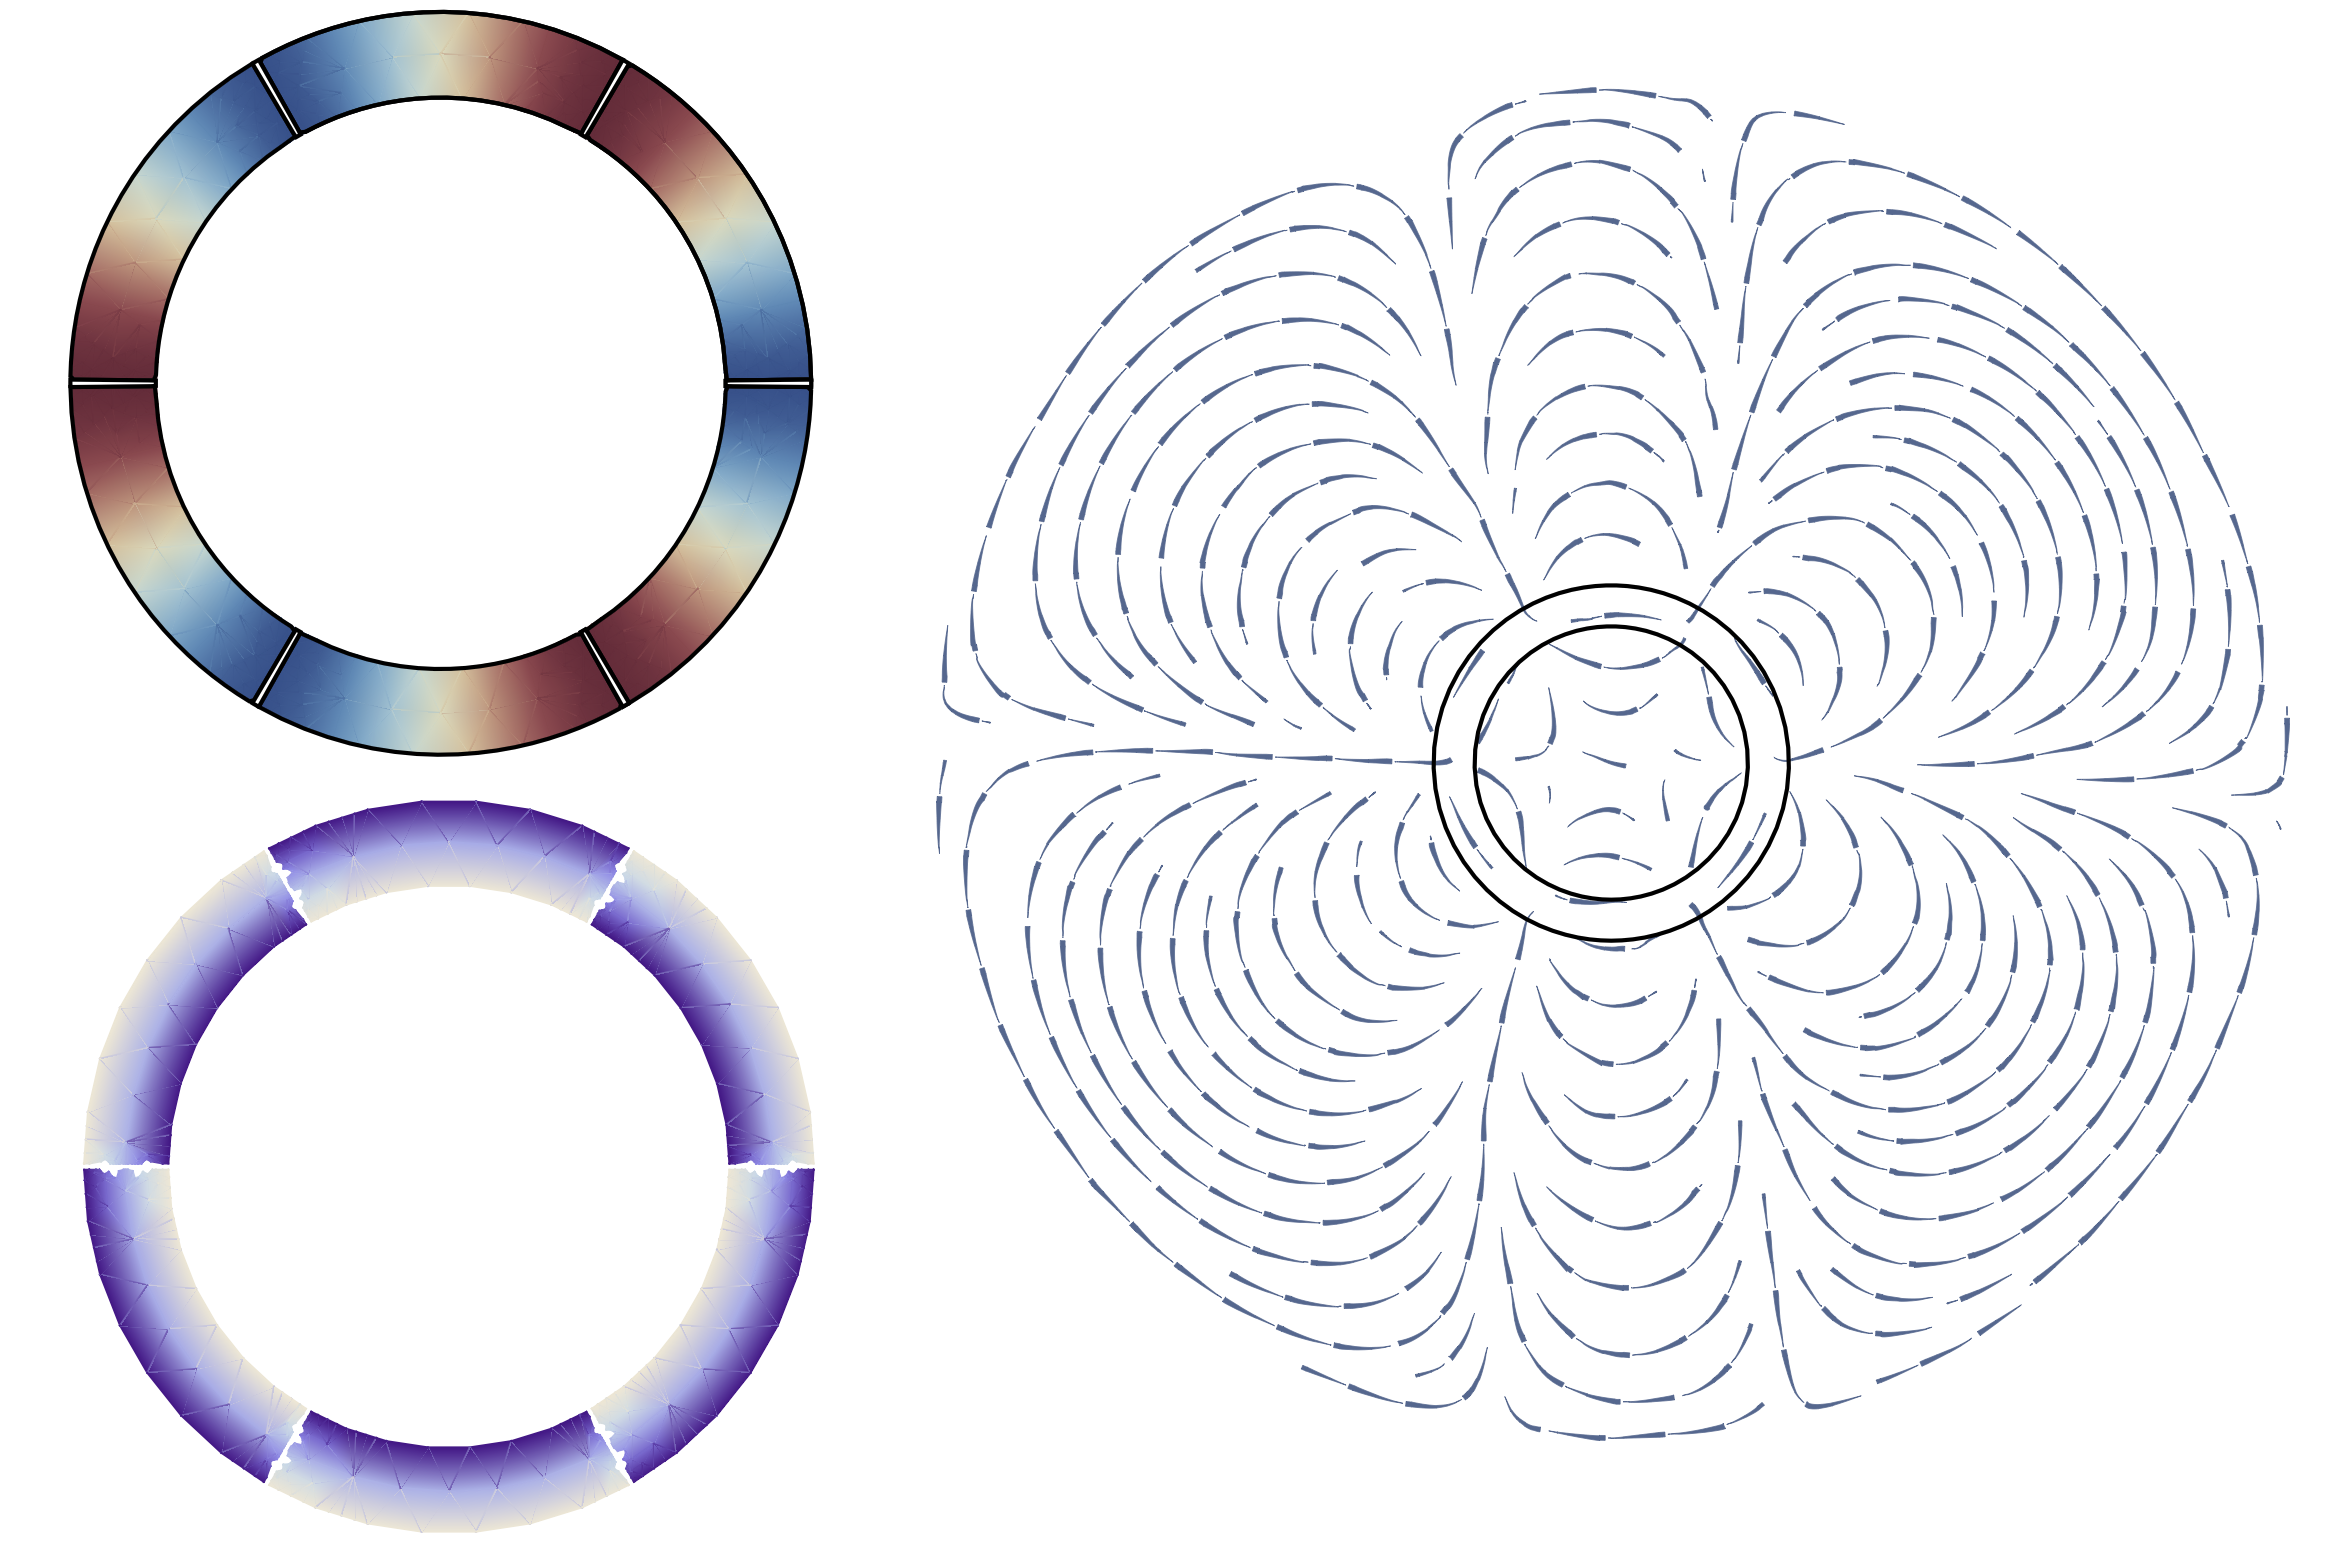
\includegraphics[width=3in]{ring.png}
        \end{center}
    \end{frame}
    \begin{frame}{Theory: Non Linear FEM}
        How can we use FEM to solve problems in the form of
        \[\nabla\cdot\left(\alpha(\|\nabla\phi\|)*\nabla\phi\right)=f(x,y)\]
        \textbf{First thing}: Determine $\|\nabla\phi\|$ on a single element in terms of node values of $\phi$: $\left( \phi_i, \phi_j, \phi_k \right)$
        \[\left|\left(\pdv{\phi}{x},\pdv{\phi}{y}\right)\right|=\left|\left(\pdv{\vec{N}}{x}, \pdv{\vec{N}}{y} \right)^{\text{T}}\cdot \left(
        \begin{array}{c}
            \phi _i \\
            \phi _j \\
            \phi _k \\
        \end{array}
        \right)\right|\]
    \end{frame}
    \begin{frame}{Solving the Non Linear System}
        Now our element matrix equation looks like:
        \[F(\vec{\phi})=\mathbf{K}\cdot\vec{\phi}*\alpha(\vec{\phi})-\vec{b}=0\]
        No more linear solver :( we need to use Newton's Method\\
        \smallbreak
        Consider the vector equation $f(\vec{x})=0$
        \begin{itemize}
            \item Start with the guess $\vec{x}\approx\vec{x}_0$
            \item Expand in power series
            \[f(\vec{x})\approx f(\vec{x}_0)+\mathbf{J}_{f(\vec{x}_0)}(\vec{x}-\vec{x}_0)\approx 0\]
            \item Solve a linear system for $\vec{x_0}$ to find a better guess for $\vec{x}$.
            Iterate.
            \begin{align*}
                &\mathbf{J}_{f(\vec{x}_n)}\left(\vec{x}_{n}-\vec{x}_{n+1}\right)=f(\vec{x}_{n})\\
                &\mathbf{J}_{F(\vec{\phi_n})}=\mathbf{K}\left( \mathbf{I}*\alpha(\vec{\phi_n})+\left(\vec{\phi_n}\right)^{\text{T}}\cdot \nabla_{\vec{\phi}}\alpha(\vec{\phi_n}) \right)\\
            \end{align*}
        \end{itemize}
    \end{frame}
    \begin{frame}{Implementation: FEA\textit{lite}}
        \hspace{-0.72cm}
        
\includegraphics[width=4.5in]{technology.pdf}

    \end{frame}

    \begin{frame}{Implementation: Mesh Generation}
        \begin{itemize}
            \item Meshes are generated using the Mathematica 12 mesh generator
            \item Exported as:\\ list of coordinates [$x$, $y$]$^v$ \\list of mesh elements [$v_1$, $v_2$, $v_3$, marker]$^{e}$ \\list of boundary elements [$v_1$, $v_2$, marker]$^{be}$
        \end{itemize}


        \begin{figure}
            \centering
            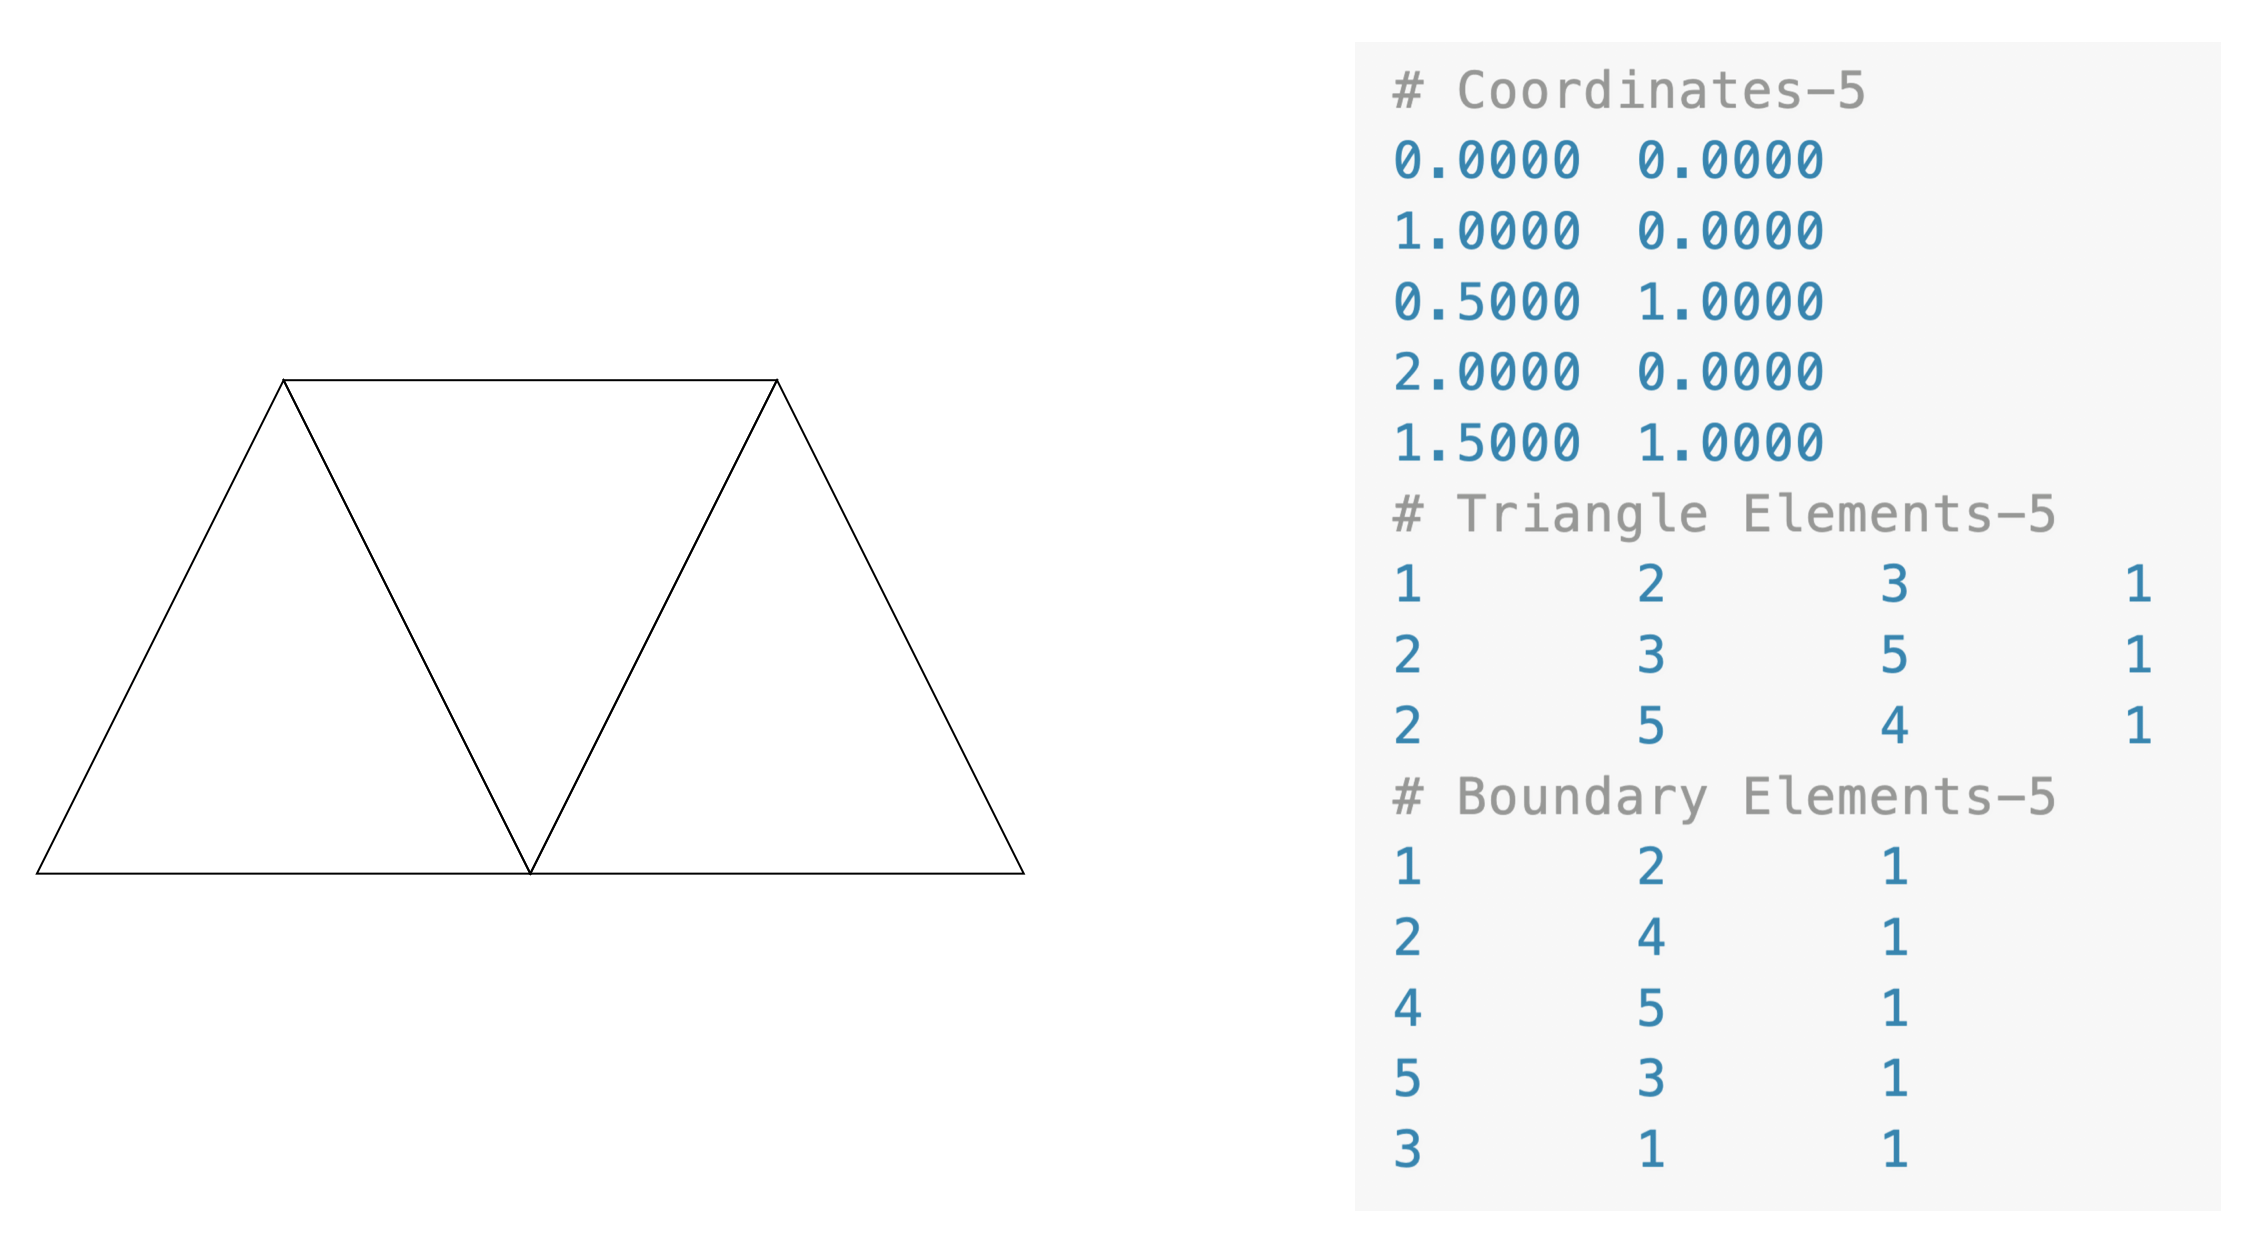
\includegraphics[width=3.5in]{meshdemo.png}
        \end{figure}

    \end{frame}
    \begin{frame}{Mesh}
        \begin{itemize}
            \item
        \end{itemize}
    \end{frame}
\end{document}
